\documentclass[12pt]{article}
\usepackage[margin=1in]{geometry}
\usepackage{setspace}
\onehalfspacing

% Start of preamble
%==========================================================================================%
% Required to support mathematical unicode
\usepackage[warnunknown, fasterrors, mathletters]{ucs}
\usepackage[utf8x]{inputenc}

\usepackage[dvipsnames,table,xcdraw]{xcolor}

% Standard mathematical typesetting packages
\usepackage{amsmath,amssymb,amscd,amsthm,amsxtra, pxfonts}
\usepackage{mathtools,mathrsfs,dsfont,xparse}

% Symbol and utility packages
\usepackage{cancel, textcomp}
\usepackage[mathscr]{euscript}
\usepackage[nointegrals]{wasysym}
\usepackage{apacite}

% Extras
\usepackage{physics}  
\usepackage{tikz-cd} 
\usepackage{microtype}
\usepackage{enumitem}
\usepackage{titling}
\usepackage{graphicx}

% Fancy theorems due to @intuitively on discord
\usepackage{mdframed}
\newmdtheoremenv[
backgroundcolor=NavyBlue!30,
linewidth=2pt,
linecolor=NavyBlue,
topline=false,
bottomline=false,
rightline=false,
innertopmargin=10pt,
innerbottommargin=10pt,
innerrightmargin=10pt,
innerleftmargin=10pt,
skipabove=\baselineskip,
skipbelow=\baselineskip
]{mytheorem}{Theorem}

\newenvironment{theorem}{\begin{mytheorem}}{\end{mytheorem}}

\newtheorem{corollary}{Corollary}
\newtheorem{lemma}{Lemma}

\newtheoremstyle{definitionstyle}
{\topsep}%
{\topsep}%
{}%
{}%
{\bfseries}%
{.}%
{.5em}%
{}%
\theoremstyle{definitionstyle}
\newmdtheoremenv[
backgroundcolor=Violet!30,
linewidth=2pt,
linecolor=Violet,
topline=false,
bottomline=false,
rightline=false,
innertopmargin=10pt,
innerbottommargin=10pt,
innerrightmargin=10pt,
innerleftmargin=10pt,
skipabove=\baselineskip,
skipbelow=\baselineskip,
]{mydef}{Definition}
\newenvironment{definition}{\begin{mydef}}{\end{mydef}}

\newtheorem*{remark}{Remark}

\newtheorem*{example}{Example}

% Common shortcuts
\def\mbb#1{\mathbb{#1}}
\def\mfk#1{\mathfrak{#1}}

\def\bN{\mbb{N}}
\def \C{\mbb{C}}
\def \R{\mbb{R}}
\def\bQ{\mbb{Q}}
\def\bZ{\mbb{Z}}
\def \cph{\varphi}
\renewcommand{\th}{\theta}
\def \ve{\varepsilon}
\newcommand{\mg}[1]{\| #1 \|}

% Often helpful macros
\newcommand{\floor}[1]{\left\lfloor#1\right\rfloor}
\newcommand{\ceil}[1]{\left\lceil#1\right\rceil}
\renewcommand{\qed}{\hfill\qedsymbol}
\renewcommand{\P}{\mathbb P\qty}
\newcommand{\E}{\mathbb{E}\qty}
\newcommand{\Cov}{\mathrm{Cov}\qty}
\newcommand{\Var}{\mathrm{Var}\qty}

% Sets
\usepackage{braket}

\graphicspath{{/}}
\usepackage{float}

\newcommand{\SET}[1]{\Set{\mskip-\medmuskip #1 \mskip-\medmuskip}}

% End of preamble
%==========================================================================================%

% Start of commands specific to this file
%==========================================================================================%

%==========================================================================================%
% End of commands specific to this file

\title{CSE 422 Hw2}
\date{\today}
\author{Rohan Mukherjee}

\begin{document}
    \maketitle
    \begin{enumerate}[leftmargin=\labelsep]
        \item
        \begin{enumerate}
            \item Here is the heatmap for Jaccard similarity first:
            \begin{figure}[H]
                \centering
                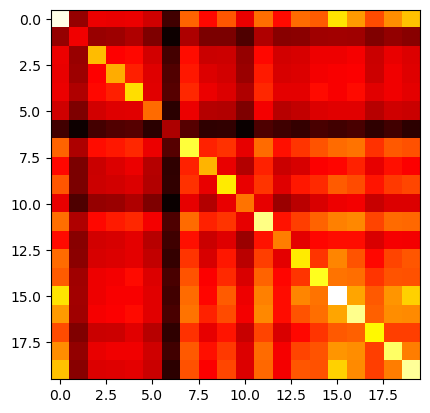
\includegraphics[width=0.5\textwidth]{jaccard_heatmap.png}
            \end{figure}
            Here is the heatmap for cosine similarity:
            \begin{figure}[H]
                \centering
                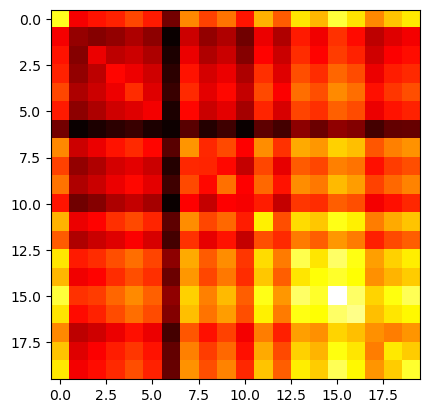
\includegraphics[width=0.5\textwidth]{cosine_heatmap.png}
            \end{figure}
            Here is the heatmap for l2 similarity:
            \begin{figure}[H]
                \centering
                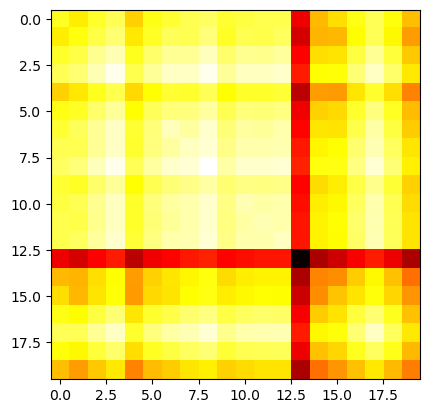
\includegraphics[width=0.5\textwidth]{l2_heatmap.png}
            \end{figure}
            \item Based on the heatmap, the Jaccard similarity does the best, followed by the cosine similarity, and finally followed by the l2 similarity. L2 just seems really bad. For one thing, I checked and it turn out with that similarity, all the groups are most simliar to group 8, whatever group 8 may be. This doesn't really make sense as the group should be most simliar to itself. Also, it seems to just think that every article is pretty related to each other, while also thinking that article 13 is really dissimiliar from itself. I think this means the articles from group 13 happen to have lots of different words (maybe synonyms), and this contributes to a very large l2 distance. 

            The cosine simliarity somehow has the same problem, where it thinks that all groups are most similar to group 15, which is christian religion. This is weird and pretty unintuitive, but I guess christian religion just uses similar words to all the groups. The issue with comparing articles to articles is that even among the same group, they could use vastly different words. 

            On the other hand, Jaccard similarity knows that the group most similar to anything else is itself. It makes all the political groups similar to each other, at least more than all the other groups. The effect is not very pronounced. It seems to like to say groups are distinct rather than similar, at least compared to the other two metrics. Interestingly, it says misc.tosale is very distinct from all the other groups. You would think it would also say all the computer related groups are similar, which it seems to do, but not nearly as pronounced as with the political groups.

            The other two metrics are kind of all over the place. L2 seems to think everything is simlar except group 15. There is a dark square around the motorcycle group, and I'm not really sure why. I didn't expect this metric to be very good.

            Cosine similarity surprised me by saying everything is most common to group 15 (christian religion). I was expecting better. For it, it also knows that political groups are very related. It like the first method doesn't make the computer groups are simliar as that one, but does seem to get similarity for the political groups more defined than the Jaccard.

            \item The l2 heatmap can be messed up really badly. For the worst possible case, I could add one article to one group that just has like $10^{100}$ of each word. Then the l2 heatmap would be really dark for that entire column, and I could continue this pattern by adding more of these huge articles to other groups. If I wanted to mess it up even further I could have these articles have dijsoint words. This would guarantee that the l2 distance is always huge between distinct groups.

            The cosine similarity is harder to mess up. This time I could add one article from each group that are most dissimilar to each other. This would then make these groups look more similar, effectively flipping the heatmap.

            On the other hand, I believe the Jaccard similarity is the most robust. It compares word usage via counts. So I could probably add the average of all the groups to each of the groups. Then this would contribute a lot to the intersection and the union would remain around the same, since they would on average all have words from this average. This would make the groups a lot more similar throwing off the pattern.

            If I was worried about these outliers, I could probably do a leave-one-out group similarity, where I compare each article $a$ from a fixed group $G$ to the articles in $G - a$. Then I would see how simliar this article is to the rest of the articles in the group. Then I would have to set some sort of arbitrary threshold to say if the article is too dissimilar to the rest of the group, remove it. This would get rid of these outliers. 
        \end{enumerate}
        
        \item
        \begin{enumerate}
            \item I have implemented it. Here is the heatmap:
            \begin{figure}[H]
                \centering
                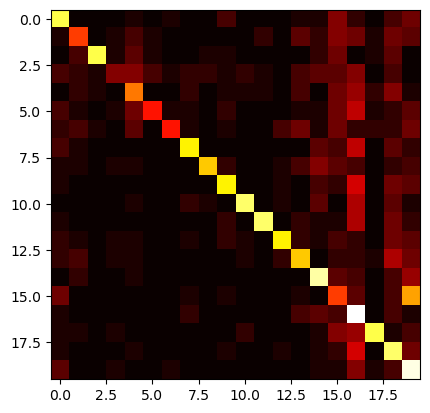
\includegraphics[width=0.5\textwidth]{heatmap_for_nns_brute.png}
            \end{figure}
            The average classification error I computed was 0.544.


            \item For each of the $n$ vectors, I find their nearest neighbor that is not them in the dataset, which requires us to compute cosine similarity with $n-1$ other vectors, where each of these computations takes the length of the vector $O(N)$ time. This gives $O(n^2N)$ time complexity.

            \item Here is the heatmap for the new algorithm, with sketch matrix having $N(0,1)$ entries:
            \begin{figure}[H]
                \centering
                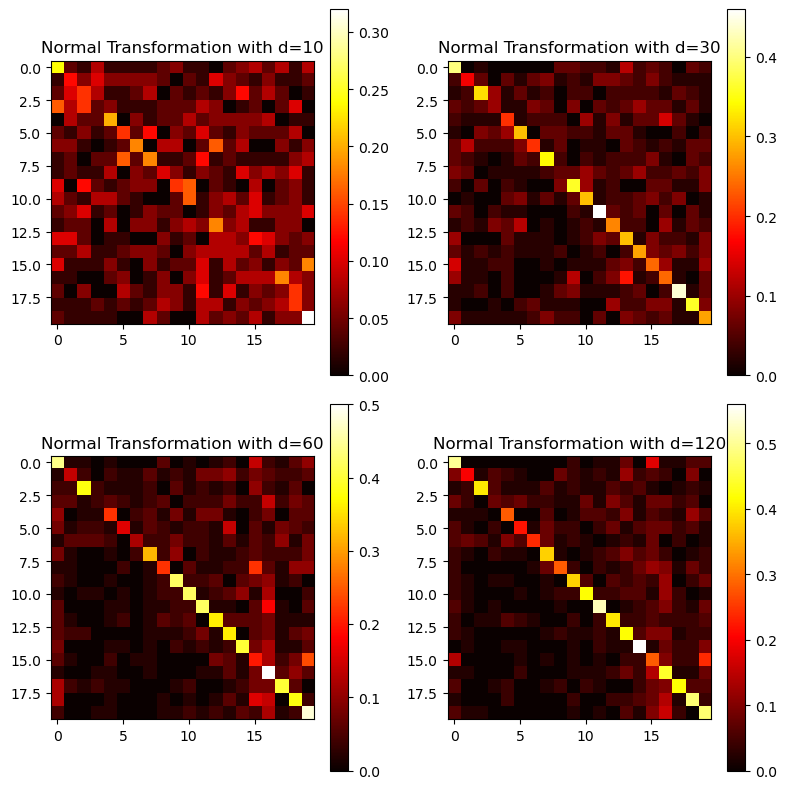
\includegraphics[width=0.5\textwidth]{normal_heatmaps.png}
            \end{figure}
            The classification error for each $d$ is as follows:
            
            \begin{table}[H]
                \centering
                \begin{tabular}{|c|c|}
                    \hline
                    \textbf{d} & \textbf{Classification Error} \\ \hline
                    10         & 0.867                         \\ \hline
                    30         & 0.720                         \\ \hline
                    60         & 0.681                         \\ \hline
                    120        & 0.631                         \\ \hline
                \end{tabular}
                \caption{Classification errors for different \( d \) for normal.}
                \label{tab:classification_errors}
            \end{table}

            For $\pm 1$ entries, we get:
            \begin{figure}[H]
                \centering
                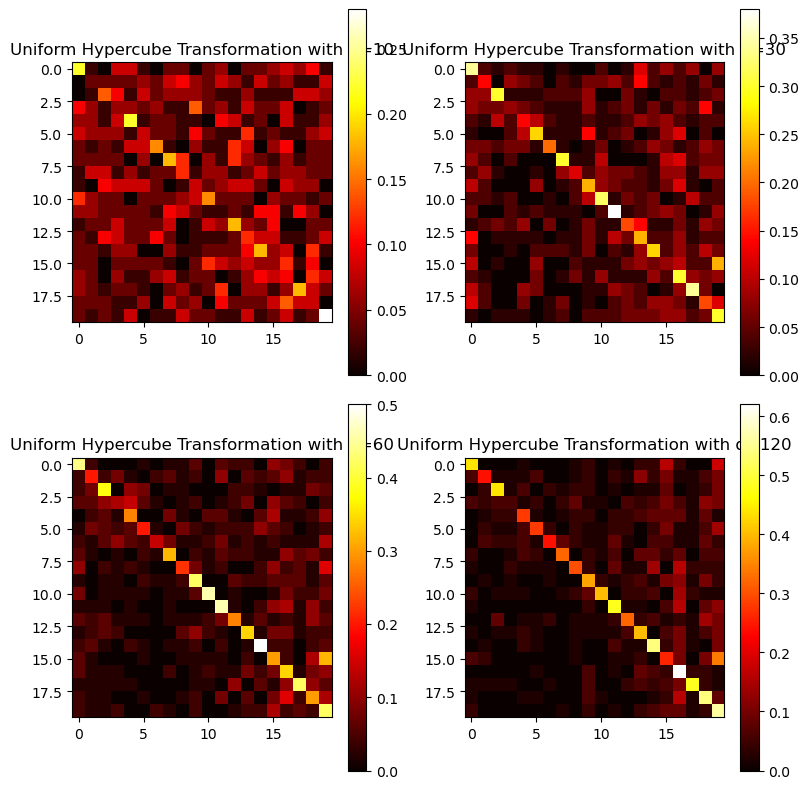
\includegraphics[width=0.5\textwidth]{uniform_heatmaps.png}
            \end{figure}
            The classification error for each $d$ is as follows:
            \begin{table}[H]
                \centering
                \begin{tabular}{|c|c|}
                    \hline
                    \textbf{d} & \textbf{Classification Error} \\ \hline
                    10         & 0.867                         \\ \hline
                    30         & 0.765                         \\ \hline
                    60         & 0.673                         \\ \hline
                    120        & 0.621                         \\ \hline
                \end{tabular}
                \caption{Classification errors for different \( d \).}
                \label{tab:classification_errors}
            \end{table}
            noticably smaller.

            For $0,1$ random entries, we get:
            \begin{figure}[H]
                \centering
                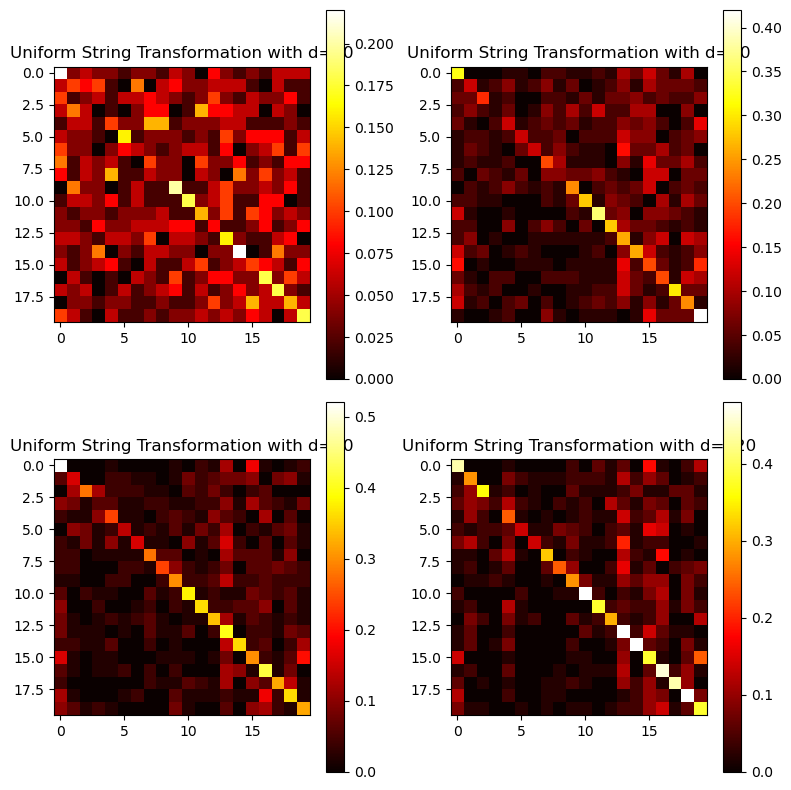
\includegraphics[width=0.5\textwidth]{string_heatmaps.png}
            \end{figure}
            with corresponding table:
            \begin{table}[H]
                \centering
                \begin{tabular}{|c|c|}
                    \hline
                    \textbf{d} & \textbf{Classification Error} \\ \hline
                    10         & 0.871                         \\ \hline
                    30         & 0.784                         \\ \hline
                    60         & 0.703                         \\ \hline
                    120        & 0.663                         \\ \hline
                \end{tabular}
                \caption{Classification errors for different \( d \).}
                \label{tab:classification_errors}
            \end{table}
            As you can see, for $d = 60$ and $d = 120$, the sketch does really well, and even sometimes better than the original dataset, which is surprising. $d = 30$ and $d = 10$ are really not very good, usually being above $0.75$, much higher than the $0.66$ the original dataset gets. 

            \item 
            As you can see, uniform does the best, normal does middle, and string does the worst. I think the main reason for this is beacuse the uniform distribution and the normal distribution have variance 1, while the string distribution has variance 0.25. This will mean that the rows of the first two methods will be more "separated" in a sense, and thus will give a better result. The string being more tightly packed will give a much worse result on the other hand. The other thing is that this method will work invariant of scaling. If we scale the matrix, we will get the same outputs. So having the samplings be able to go $+\infty$, as with $N(0,1)$ can be potentially worse, since we could get large variance from really large values but not actually separated rows. On the other hand, the $\pm 1$ distribution attains good variance while being bounded, assuring that the rows are separated as possible, without having to worry as much about scaling. 

            \item For the new algorithm, we have to compute the sketch matrix against all the $n$ vectors, who all have length $N$, so for each vector this takes a $1 \times N$ matrix multiplying $N \times d$ which takes $O(Nd)$ time, which we do a total of $n$ times. So we get the pre-processing step of$ O(nNd)$ time. Then we just do the same algorithm as before but the cosine similarity takes only $O(d)$ time to compute for each pair of vectors, yielding $O(Nnd + n^2d)$ time. This is much, much faster, especially when considering that $N$ is on the order of 68,000 and $d$ is only like 120.

            \item If we had a fixed matrix $M \in \R^{d \times N}$, then its kernel would have dimension at least $N-d$ by rank nullity. If we take a basis of $N-d$ vectors, we could transform this basis to be in $m$ distinct clusters that are very close to each other. But then $M$ would just map the entire dataset to 0, so we would lose all information about distance between them. On the otehr hand, for any article $x \in \R^N$, a random matrix should have full rank $d$. Then the kernel would have dimension $N-d$, which has measure 0, not being full in dimension. Thus the probabilty that any of our vectors is in the kernel is 0 for random matrices, thus avoiding this issue almost surely.
        \end{enumerate}
    \end{enumerate}
\end{document}